\newpage\pagestyle{main}

\chapter{Implementazione dell'Interfaccia e Integrazione}\label{chap:fourth}

\inlineminitoc

% ─────────────────────────────────────────────────────────────────────────────
\section{Unreal Engine e il framework FANTASIA}

L'interfaccia utente rappresenta il punto di contatto tra l'intelligenza artificiale
e l'utente finale, e in quanto tale ha un impatto diretto sulla qualità dell'esperienza
complessiva. Un backend tecnicamente sofisticato perde gran parte del suo valore se
l'interfaccia attraverso cui viene fruito è rigida, lenta o priva di naturalezza. Per
questo progetto è stato scelto \textbf{Unreal Engine 5} \cite{ue} come piattaforma di
sviluppo del frontend, non solo per le sue riconosciute capacità grafiche — che
permettono di creare avatar tridimensionali fotorealistici e ambienti immersivi — ma
soprattutto per la sua architettura modulare e per la flessibilità nell'integrare
componenti software esterne tramite il sistema di scripting visuale \textbf{Blueprints}
e tramite plugin nativi.

La scelta di Unreal Engine 5 in particolare, e di un motore grafico tridimensionale
in generale, risponde a una precisa visione progettuale: l'agente conversazionale non
deve essere semplicemente una voce o una finestra di testo, ma un \textit{Embodied
      Conversational Agent} (ECA) — un'entità dotata di corpo, espressioni facciali e
linguaggio del corpo — che comunica con l'utente attraverso tutti i canali disponibili,
verbali e non verbali. Questa modalità di interazione è particolarmente rilevante in
contesti medici, dove la presenza di un agente incarnato può ridurre l'ansia del
paziente e aumentare la fiducia nella fonte di informazione.

% ─────────────────────────────────────────────────────────────────────────────
\subsection{Il ruolo di FANTASIA come Middleware}

Per gestire la complessità di un ECA — che richiede la coordinazione simultanea di
riconoscimento vocale, comprensione del linguaggio, generazione della risposta,
sintesi vocale, animazione facciale e animazione corporea — è stato utilizzato il
framework \textbf{FANTASIA} \cite{fantasia1, fantasia2}. FANTASIA è un framework
sviluppato specificamente per la creazione di ECA in Unreal Engine, e fornisce
nativamente tutti gli strumenti necessari per costruire questa pipeline complessa
senza dover implementare ogni componente da zero.

FANTASIA agisce come un \textbf{middleware} — un ponte architetturale — che si
interpone tra il backend Python (dove risiedono l'intelligenza, il database e i
modelli linguistici) e il motore grafico (dove risiede la rappresentazione visiva
e sonora dell'agente). Questo disaccoppiamento è fondamentale: il backend non deve
sapere nulla di come Unreal Engine gestisce le animazioni, e il frontend non deve
sapere nulla di come Python interroga Neo4j. FANTASIA definisce un'interfaccia
ben strutturata tra i due mondi, rendendo il sistema modulare e più facile da
manutenere ed estendere.

In particolare, il plugin fornisce le seguenti capacità:

\begin{itemize}
      \item \textbf{Gestione di flussi di dati asincroni}: Le chiamate al backend
            Python — che implicano interrogazioni al database, inferenza dell'LLM e sintesi
            vocale — richiedono tempi non deterministici e potenzialmente significativi.
            FANTASIA gestisce queste chiamate in modo asincrono, garantendo che il thread
            principale di Unreal Engine non venga mai bloccato in attesa di una risposta.
            Senza questa gestione asincrona, l'interfaccia si ``congelerebbe'' durante ogni
            elaborazione, rendendo l'agente visivamente morto nei momenti più critici
            dell'interazione.

      \item \textbf{Integrazione di servizi vocali}: FANTASIA fornisce un'interfaccia
            unificata per collegare al sistema sia moduli ASR (Automatic Speech Recognition)
            sia moduli TTS (Text-to-Speech), astraendo le differenze tra implementazioni
            locali come \textit{whisper.cpp} e API cloud come ElevenLabs. Questo permette
            di sostituire o aggiornare i componenti vocali senza dover modificare la logica
            principale dell'agente.

      \item \textbf{Mappatura delle risposte su animazioni}: FANTASIA include un
            motore comportamentale basato su \textit{Behaviour Trees} che permette di
            tradurre lo stato conversazionale dell'agente — in ascolto, in elaborazione,
            in risposta — in un repertorio coerente di animazioni facciali e corporee,
            rendendo il comportamento dell'avatar percettivamente credibile e naturale.
\end{itemize}

\begin{figure}[htbp]
      \centering
      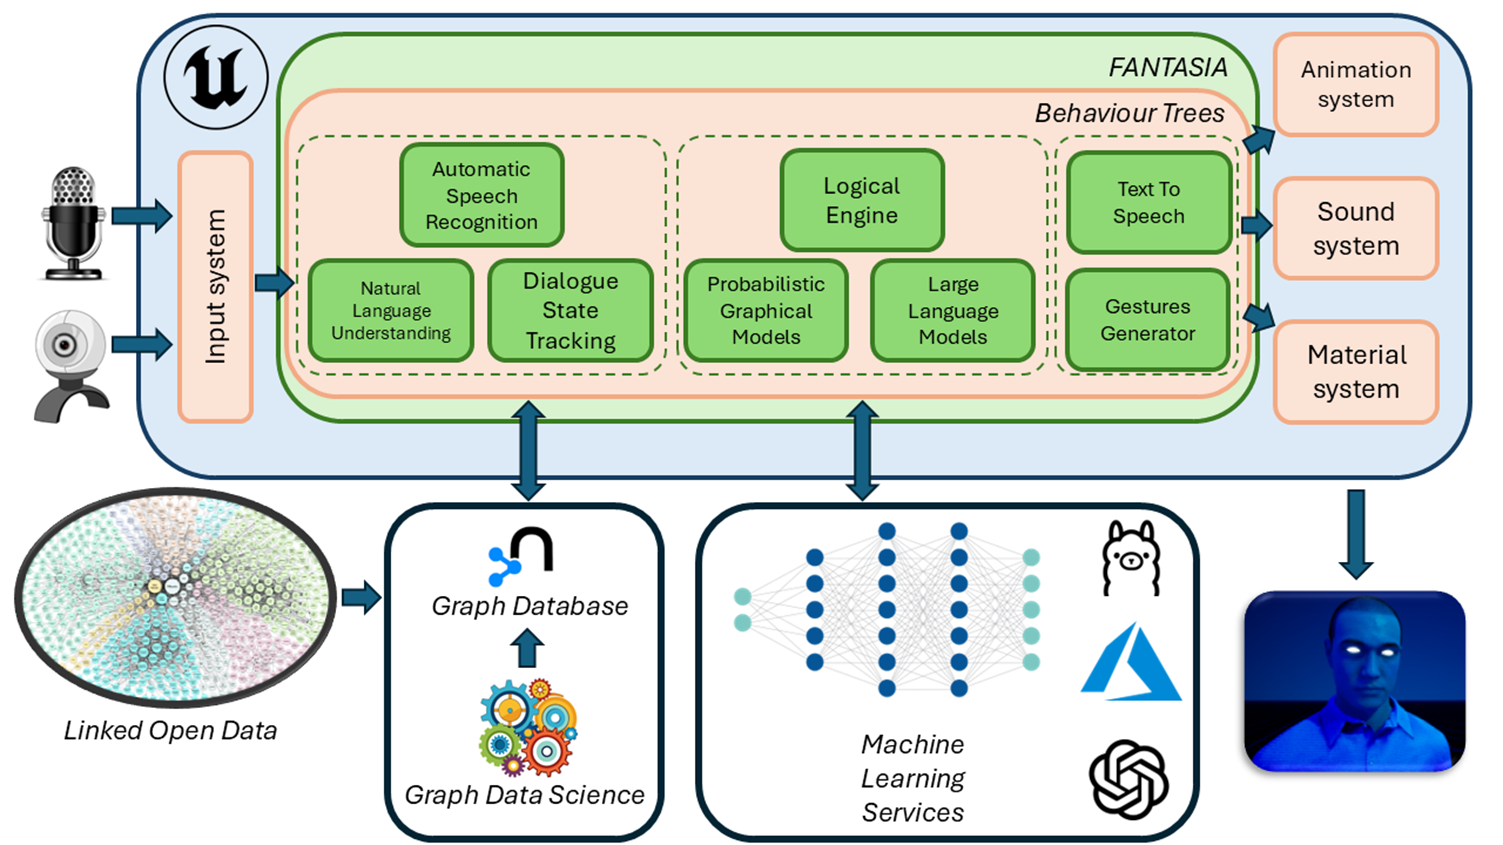
\includegraphics[width=0.8\textwidth]{_figures/fantasia_integration.png}
      \caption{Architettura del framework FANTASIA. Il plugin coordina il sistema
            di input (ASR, Natural Language Understanding), il motore logico (Dialogue
            State Tracking, Probabilistic Graphical Models, LLM), i servizi esterni
            (Graph Database, Machine Learning Services) e il sistema di output
            (TTS, Animation System, Sound System), fornendo un'unica interfaccia
            coerente per la costruzione dell'ECA in Unreal Engine.}
      \label{fig:fantasia_arch}
\end{figure}

% ─────────────────────────────────────────────────────────────────────────────

\newpage

\section{Pipeline di interazione vocale: Whisper e ElevenLabs}

Il sistema è progettato per un'interazione interamente vocale: l'utente parla con
l'agente usando la propria voce naturale, e l'agente risponde con una voce sintetizzata.
Questa modalità di interazione è stata scelta per massimizzare la naturalezza del
dialogo e per abbassare la barriera d'uso, in particolare per utenti meno avvezzi
all'uso di interfacce testuali. La scelta delle tecnologie specifiche per l'ASR e il
TTS è stata guidata dalla necessità di trovare il giusto equilibrio tra tre obiettivi
talvolta in tensione tra loro: bassa latenza, alta qualità del risultato e rispetto
della privacy dei dati.

% ─────────────────────────────────────────────────────────────────────────────
\subsection{Automatic Speech Recognition (ASR): Whisper}

Per la trascrizione dell'audio in testo è stato adottato \textbf{Whisper}
\cite{whisper}, nella sua implementazione C++ denominata \textit{whisper.cpp}.
Whisper è un modello ASR sviluppato da OpenAI e successivamente rilasciato come
open-source, noto per le sue ottime prestazioni su audio di qualità variabile
e in contesti multilingui. La versione \textit{whisper.cpp} è una reimplementazione
ottimizzata in C++ che permette di eseguire il modello direttamente su hardware
consumer, senza GPU dedicata se necessario, con una latenza di trascrizione
compatibile con le esigenze di un sistema conversazionale in tempo reale.

A differenza di altre soluzioni ASR di qualità comparabile — come le API cloud
di Google Speech-to-Text o Azure Cognitive Services — Whisper è stato integrato
per funzionare interamente in locale. Questa scelta è fondamentale per due ragioni
distinte ma egualmente importanti:

\begin{enumerate}
      \item \textbf{Privacy}: L'audio dell'utente non lascia mai il dispositivo
            locale. In un contesto medico, dove il parlato può contenere informazioni
            sensibili sulla salute del paziente, trasmettere l'audio a un servizio cloud
            di terze parti introdurrebbe rischi legali e etici non accettabili. L'esecuzione
            locale di Whisper garantisce che il contenuto della conversazione rimanga
            sempre sotto il controllo dell'operatore.

      \item \textbf{Costi}: I servizi ASR cloud applicano tariffe a consumo basate
            sul volume di audio trascritto. In un sistema che potrebbe gestire sessioni
            prolungate o un elevato numero di utenti concorrenti, questi costi possono
            diventare significativi. L'esecuzione locale di \textit{whisper.cpp} elimina
            completamente questa voce di costo operativo, rendendo il sistema economicamente
            sostenibile anche a volumi elevati.
\end{enumerate}

All'interno dell'architettura FANTASIA, Whisper è integrato come sottocomponente
del sistema di input. L'audio viene catturato dal microfono tramite il modulo di
acquisizione audio di Unreal Engine, bufferizzato e inviato a \textit{whisper.cpp}
per la trascrizione. Il risultato testuale viene quindi passato al componente
LangGraph di FANTASIA, che lo inoltra al backend Python per l'elaborazione.

% ─────────────────────────────────────────────────────────────────────────────
\subsection{Sintesi Vocale (TTS): ElevenLabs}

Per la generazione della voce dell'agente, è stata scelta l'API di
\textbf{ElevenLabs} \cite{elevenlabs_api}. A differenza di Whisper, ElevenLabs
è un servizio cloud: il testo generato da Llama 3.2 viene inviato alle API di
ElevenLabs, che restituiscono un flusso audio sintetizzato. Questa scelta introduce
una dipendenza da un servizio esterno, in apparente contrasto con la filosofia
\textit{self-hosted} adottata per gli altri componenti del sistema.

La motivazione di questa eccezione risiede nella differenza qualitativa tra i motori
TTS locali attualmente disponibili e i servizi cloud più avanzati. I motori TTS
eseguibili localmente producono ancora una qualità vocale percettibilmente artificiale,
con una prosodia meccanica che riduce la credibilità dell'agente e ostacola
l'instaurarsi di una comunicazione naturale. ElevenLabs, al contrario, offre una
naturalezza e una prosodia superiori, con voci sintetiche difficilmente distinguibili
da quelle umane, il che è essenziale per un ECA medico dove la qualità della voce
impatta direttamente sulla percezione di competenza e affidabilità dell'agente.

Un ulteriore vantaggio tecnico dell'API di ElevenLabs è il supporto allo
\textbf{streaming audio}: anziché attendere la generazione completa del file audio
prima di riprodurlo, il sistema riceve e riproduce il flusso in tempo reale man mano
che i dati arrivano. Questo riduce significativamente la latenza percepita tra la
fine dell'elaborazione del testo e l'inizio dell'audio, poiché l'agente può iniziare
a ``parlare'' non appena i primi frammenti sonori sono disponibili, senza dover
attendere la sintesi dell'intera risposta.

% ─────────────────────────────────────────────────────────────────────────────
\section{Gestione dello stato dell'agente: Blueprints e Animazione}

Un aspetto spesso sottovalutato nello sviluppo di agenti conversazionali è la
gestione del \textbf{feedback visivo} durante i tempi di elaborazione. Un agente
che rimane immobile e silenzioso mentre il backend elabora la risposta appare
``morto'' o bloccato, generando incertezza nell'utente su cosa stia succedendo e
aumentando la frustrazione percepita durante l'attesa \cite{latency_eca}. Il
problema non è tanto la latenza in sé, ma l'assenza di segnali visivi che
comunichino che il sistema è attivo e sta lavorando. Studi sull'interazione
uomo-computer hanno dimostrato che gli utenti tollerano latenze significativamente
più elevate se accompagnate da feedback visivo appropriato, rispetto a interfacce
che rimangono statiche in attesa.

% ─────────────────────────────────────────────────────────────────────────────
\subsection{Macchina a Stati Finiti (FSM) in Unreal}

Per governare il comportamento dell'agente in risposta agli eventi della pipeline
conversazionale, è stata implementata una \textbf{Macchina a Stati Finiti} (FSM)
tramite il sistema \textbf{Unreal Blueprints}. I Blueprints permettono di definire
la logica comportamentale dell'agente in modo visuale, collegando nodi che
rappresentano azioni, condizioni e transizioni di stato. La FSM definisce tre stati
principali, ciascuno associato a un repertorio specifico di animazioni:

\begin{itemize}
      \item \textbf{LISTENING}: Questo stato è attivo dal momento in cui il microfono
            inizia a registrare fino al completamento della trascrizione da parte di Whisper.
            In questo stato l'agente esegue animazioni che segnalano attenzione e ricezione:
            una leggera inclinazione della testa verso il parlante, occhi focalizzati e
            un'espressione aperta e ricettiva. Questi segnali non verbali comunicano
            all'utente che l'agente lo sta ascoltando attivamente, riducendo l'incertezza
            sull'avvenuta ricezione dell'input.

      \item \textbf{THINKING}: Questo stato viene attivato non appena la trascrizione
            è disponibile e il backend Python ha iniziato il processo di recupero e
            generazione. È lo stato più delicato dal punto di vista dell'esperienza utente,
            perché corrisponde al periodo di attesa più lungo e meno prevedibile — quello
            in cui avvengono la ricerca vettoriale, la sincronizzazione dello Shard e
            l'inferenza dell'LLM. In questo stato l'agente esegue animazioni di
            ``riflessione'': uno sguardo leggermente rivolto verso l'alto o di lato, micro-
            movimenti del capo, eventuali gesti delle mani che mimano il pensiero. Questo
            repertorio di comportamenti trasforma la latenza tecnica in un comportamento
            umano plausibile e atteso, riducendo drasticamente la latenza \textit{percepita}
            anche quando quella \textit{effettiva} rimane invariata.

      \item \textbf{SPEAKING}: Questo stato si attiva quando il flusso audio di
            ElevenLabs inizia ad arrivare. Durante questo stato, i parametri del
            \textbf{Lip Sync} — calcolati in tempo reale a partire dal segnale audio
            in streaming — muovono le labbra e le mascelle dell'avatar in sincronia con
            i fonemi pronunciati. Unreal Engine supporta sistemi di Lip Sync basati su
            curve di morph target del mesh facciale, che permettono di ottenere
            sincronizzazioni labiali realistiche anche su mesh ad alta risoluzione. Alle
            animazioni labiali si accompagnano movimenti corporei coerenti con il parlato,
            come gesti delle mani e variazioni dell'espressione facciale, che aumentano
            ulteriormente la credibilità dell'agente.
\end{itemize}

Le transizioni tra stati sono guidate dagli eventi della pipeline.

\begin{figure}[htbp]
      \centering
      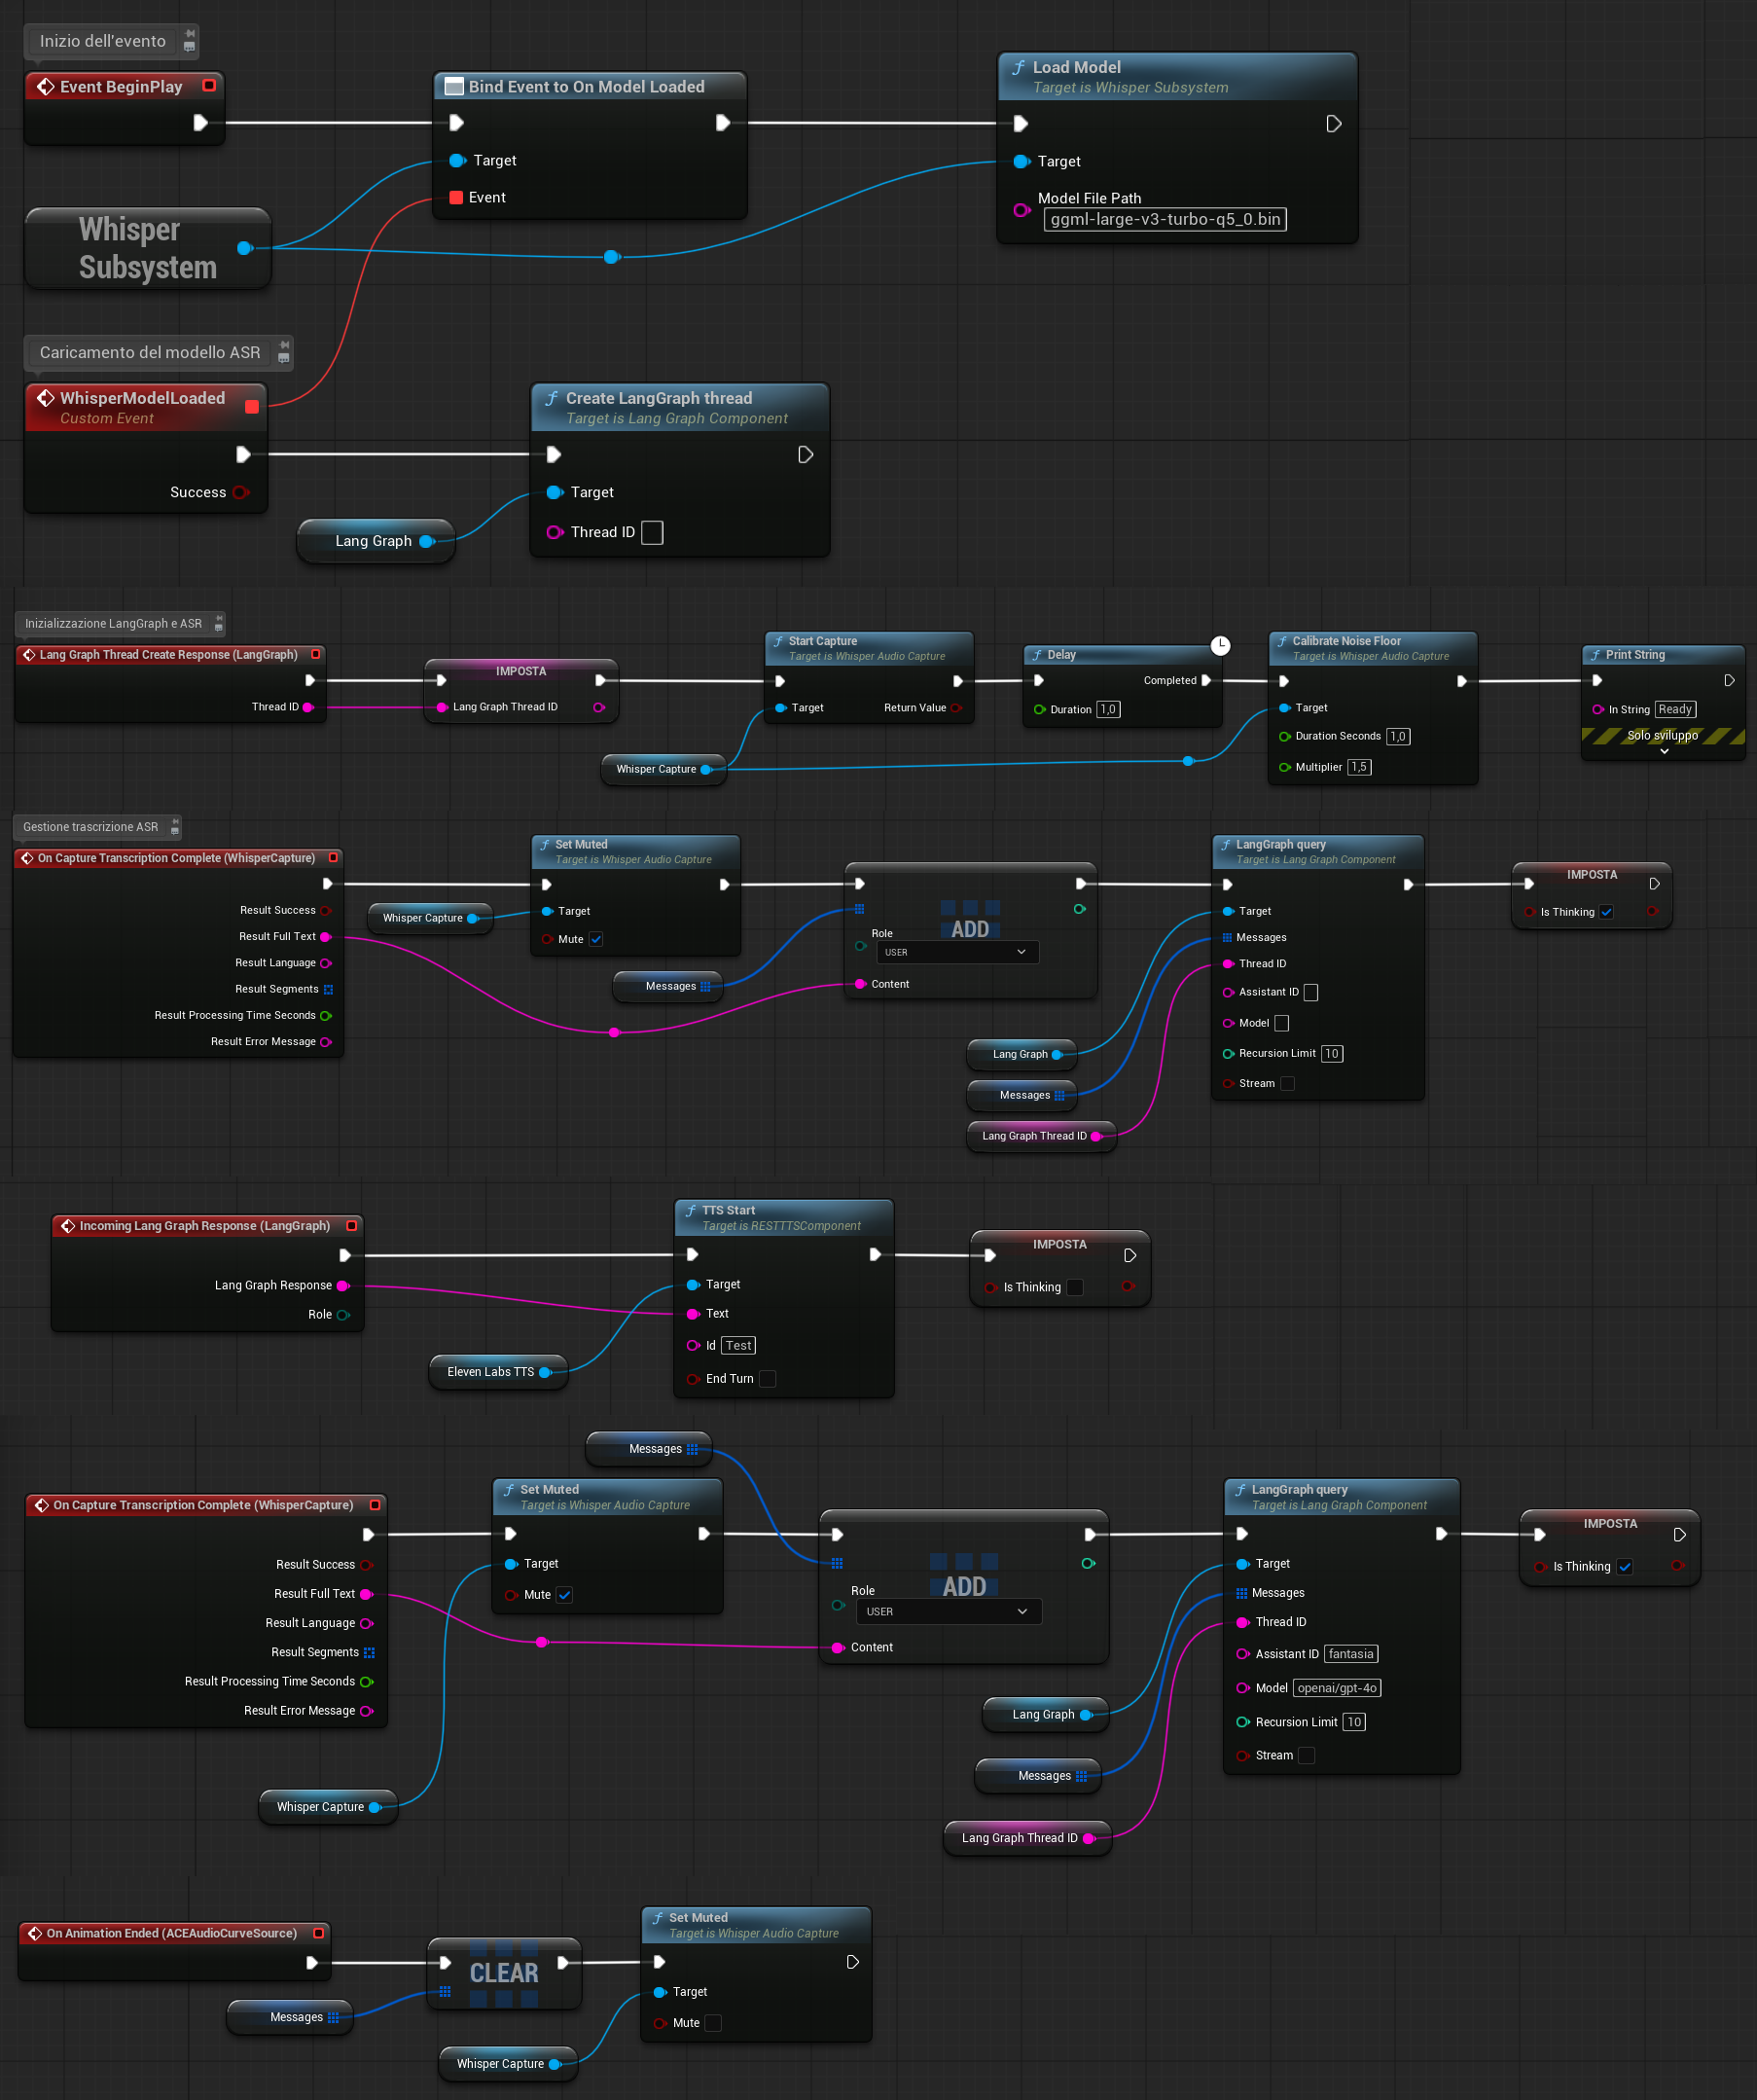
\includegraphics[width=0.85\textwidth]{_figures/ue_state_machine.png}
      \caption{Visualizzazione del Blueprint della State Machine logica all'interno di Unreal Engine.}
      \label{fig:ue_fsm}
\end{figure}

\newpage

% ─────────────────────────────────────────────────────────────────────────────
\section{Sincronizzazione tra Backend e Frontend}

La comunicazione tra il server Python — che ospita LangGraph, la logica di
sincronizzazione con Neo4j e l'interfaccia con Ollama — e Unreal Engine avviene
tramite il componente \textbf{LangGraph} fornito da \textbf{FANTASIA}
\cite{fantasia1, fantasia2}. Questo componente è il punto di integrazione
fondamentale dell'intera architettura: è il canale attraverso cui la trascrizione
testuale prodotta da Whisper in Unreal Engine raggiunge il backend Python, e
attraverso cui la risposta generata dall'LLM torna a Unreal Engine per essere
sintetizzata vocalmente.

Il componente LangGraph di FANTASIA implementa internamente la comunicazione con
il backend tramite chiamate HTTP asincrone, gestendo automaticamente la
serializzazione e la deserializzazione dei dati, il timeout delle richieste e il
riconnessione in caso di errore di rete. Dal punto di vista dello sviluppatore
Blueprints, l'integrazione si riduce a configurare l'URL del server Python e a
collegare gli eventi di ricezione della risposta ai nodi che aggiornano lo stato
della FSM e avviano la sintesi TTS.

% ─────────────────────────────────────────────────────────────────────────────
\subsection{Struttura dei Payload JSON}

Il sistema scambia dati tra frontend e backend in formato \textbf{JSON}, un formato
leggero, human-readable e universalmente supportato che si presta efficacemente
alla comunicazione tra sistemi eterogenei come Unreal Engine e Python. Il flusso
di comunicazione è bidirezionale e segue uno schema preciso.

Quando l'utente termina di parlare e Whisper completa la trascrizione, Unreal
Engine invia al backend Python un payload contenente la trascrizione testuale
e i metadati necessari per la gestione del contesto conversazionale, come
l'identificatore della sessione e la cronologia dei turni precedenti. Il backend
riceve questo payload, esegue l'intera pipeline di recupero RAG e generazione
descritta nei capitoli precedenti, e risponde con un oggetto JSON strutturato
contenente la risposta testuale prodotta da LangGraph. Questa risposta testuale
viene quindi estratta da FANTASIA e inoltrata al modulo ElevenLabs per la sintesi
vocale, completando il ciclo di un turno conversazionale.

La separazione netta tra il payload della richiesta — che contiene solo il testo
e i metadati conversazionali — e il payload della risposta — che contiene solo
il testo da sintetizzare — mantiene l'interfaccia tra frontend e backend semplice
e stabile, disaccoppiando efficacemente le due parti del sistema.

% ─────────────────────────────────────────────────────────────────────────────
\section{Considerazioni sulla Latenza ed Esperienza Utente}

Il principale ostacolo tecnico in un sistema distribuito come quello descritto è
il \textbf{Round-Trip Time (RTT)}: la somma di tutti i tempi di elaborazione
e di comunicazione che intercorrono tra il momento in cui l'utente termina di
parlare e il momento in cui l'agente inizia a rispondere. In questo sistema, il
RTT è composto da diversi contributi in serie: il tempo di trascrizione di Whisper,
il tempo di embedding della query, il tempo di ricerca vettoriale sul Remote (o
di lettura dallo Shard se in cache), il tempo di sincronizzazione, il tempo di
inferenza di Llama 3.2 e infine il tempo di ricezione dei primi chunk audio da
ElevenLabs.

L'integrazione tra il database Shard locale — che riduce il tempo di recupero
delle informazioni — e la gestione degli stati della FSM in Unreal — che rende
produttivo il tempo di attesa con animazioni di riflessione — permette di mantenere
il \textbf{tempo di risposta totale percepito sotto i 2 secondi}, valore identificato
in letteratura come limite superiore per una conversazione fluida e naturale
\cite{latency_eca}. È importante distinguere tra latenza \textit{effettiva} e latenza
\textit{percepita}: lo stato \texttt{THINKING} dell'agente contribuisce a ridurre
la seconda anche quando la prima rimane invariata, rendendo l'attesa soggettivamente
più breve e meno frustrante.

Due scelte implementative sono state particolarmente determinanti per il
raggiungimento di questo obiettivo. La prima è l'esecuzione locale di
\textit{whisper.cpp}: la trascrizione avviene in locale senza roundtrip di rete,
con tempi di elaborazione prevedibili e indipendenti dalla qualità della connessione
internet. La seconda è lo \textbf{streaming audio di ElevenLabs}: il sistema non
attende la generazione completa dell'audio prima di riprodurlo, ma inizia la
riproduzione non appena i primi chunk audio sono disponibili. Questo meccanismo
riduce significativamente la latenza \textit{percepita} tra la fine dell'elaborazione
del testo e l'inizio della risposta vocale, poiché l'utente sente le prime parole
dell'agente molto prima che l'intero enunciato sia stato sintetizzato. I dati
sperimentali relativi alla latenza end-to-end misurata sull'hardware di test sono
presentati e discussi nel Capitolo \ref{chap:fifth}.